% 3,5,6,7,8

%\pagebreak


\aufgabe{}{5}

Sketch a simple model of a real-time system and partition it into three important parts. 
Name each cluster and the interfaces between them.

\begin{tikzpicture}
\node (rect) at (0,0) [draw, text width=17 cm, minimum height=16cm]{};
\node[below right, text width=17 cm] at (rect.north west) {
    \lsg{
    Please sketch a model here
    }
   };
\end{tikzpicture}

\pagebreak

\headheight = 78pt

\aufgabe{}{2}

What is a history state? Please explain with an example.

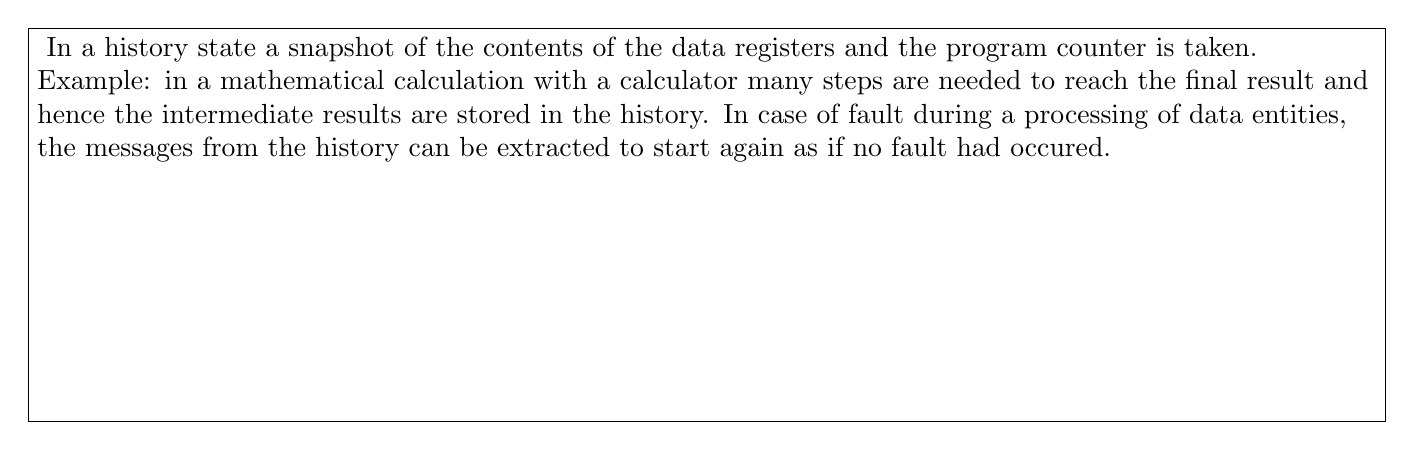
\begin{tikzpicture}
\node (rect) at (0,0) [draw, text width=17 cm, minimum height=5cm]{};
\node[below right, text width=17cm] at (rect.north west) {
    \lsg{
    In a history state a snapshot of the contents of the data registers and the program counter is taken. \\
    Example: in a mathematical calculation with a calculator many steps are needed to reach the final result and hence the intermediate results
    are stored in the history. In case of fault during a processing of data entities, the messages from the history can be extracted to start again as if no fault had occured.
    }
   };
\end{tikzpicture}

\aufgabe{}{1}

What does signal conditioning mean? Give an example.

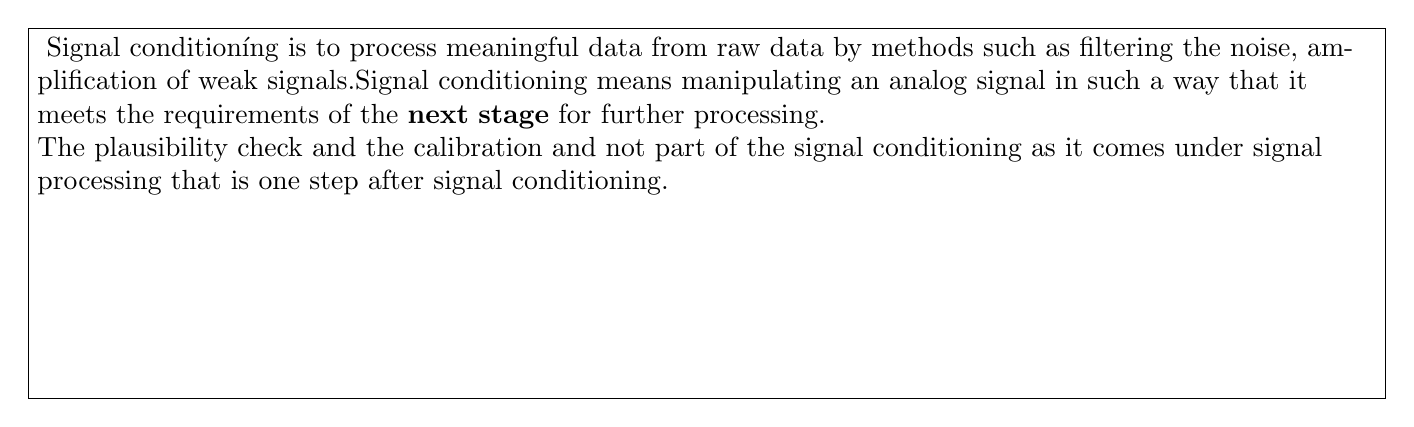
\begin{tikzpicture}
\node (rect) at (0,0) [draw, text width=17 cm, minimum height=4.7cm]{};
\node[below right, text width=17 cm] at (rect.north west) {
    \lsg{
    Signal conditioníng is to process meaningful data from raw data by methods such as filtering the noise, amplification of weak signals.Signal conditioning means manipulating an analog signal in such a way that it meets the requirements of the \textbf{next stage} for further processing.\\
		The plausibility check and the calibration and not part of the signal conditioning as it comes under signal processing that is one step after signal conditioning. 
    }
   };
\end{tikzpicture}

\aufgabe{}{1}

Explain the difference between polling and sampling.

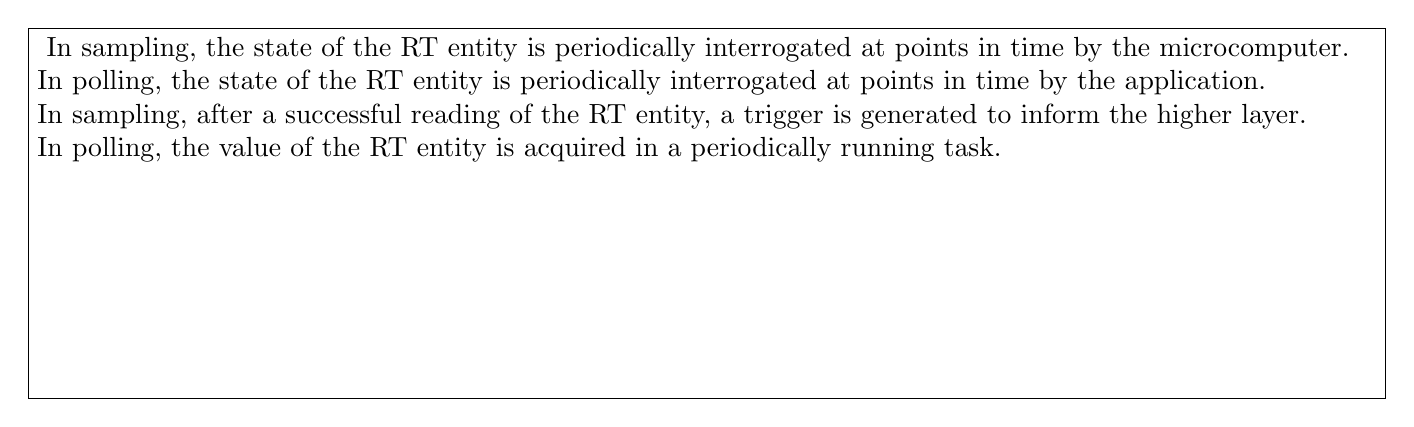
\begin{tikzpicture}
\node (rect) at (0,0) [draw, text width=17 cm, minimum height=4.7cm]{};
\node[below right, text width=17 cm] at (rect.north west) {
    \lsg{ 
    In sampling, the state of the RT entity is periodically interrogated at points in time by the microcomputer. \\
    In polling, the state of the RT entity is periodically interrogated at points in time by the application. \\
    In sampling, after a successful reading of the RT entity, a trigger is generated to inform the higher layer. \\
    In polling, the value of the RT entity is acquired in a periodically running task.
    }
   };
\end{tikzpicture}

\pagebreak


\aufgabe{}{1}


Consider a combustion engine with an injection valve. The start point of fuel injection must 
be precise within 0.1 $\deg$ of the measured angular crankshaft position.
Calculate the temporal accuracy of the system if the crankshaft revolves with 6000 rpm.


\begin{tikzpicture}
\node (rect) at (0,0) [draw, text width=17 cm, minimum height=5cm]{};
\node[below right, text width=17 cm] at (rect.north west) {
    \lsg{
    2.7 $\mu$s
    }
   };
\end{tikzpicture}

\aufgabe{}{5}

Define offset, drift, drift rate, precision, and accuracy.


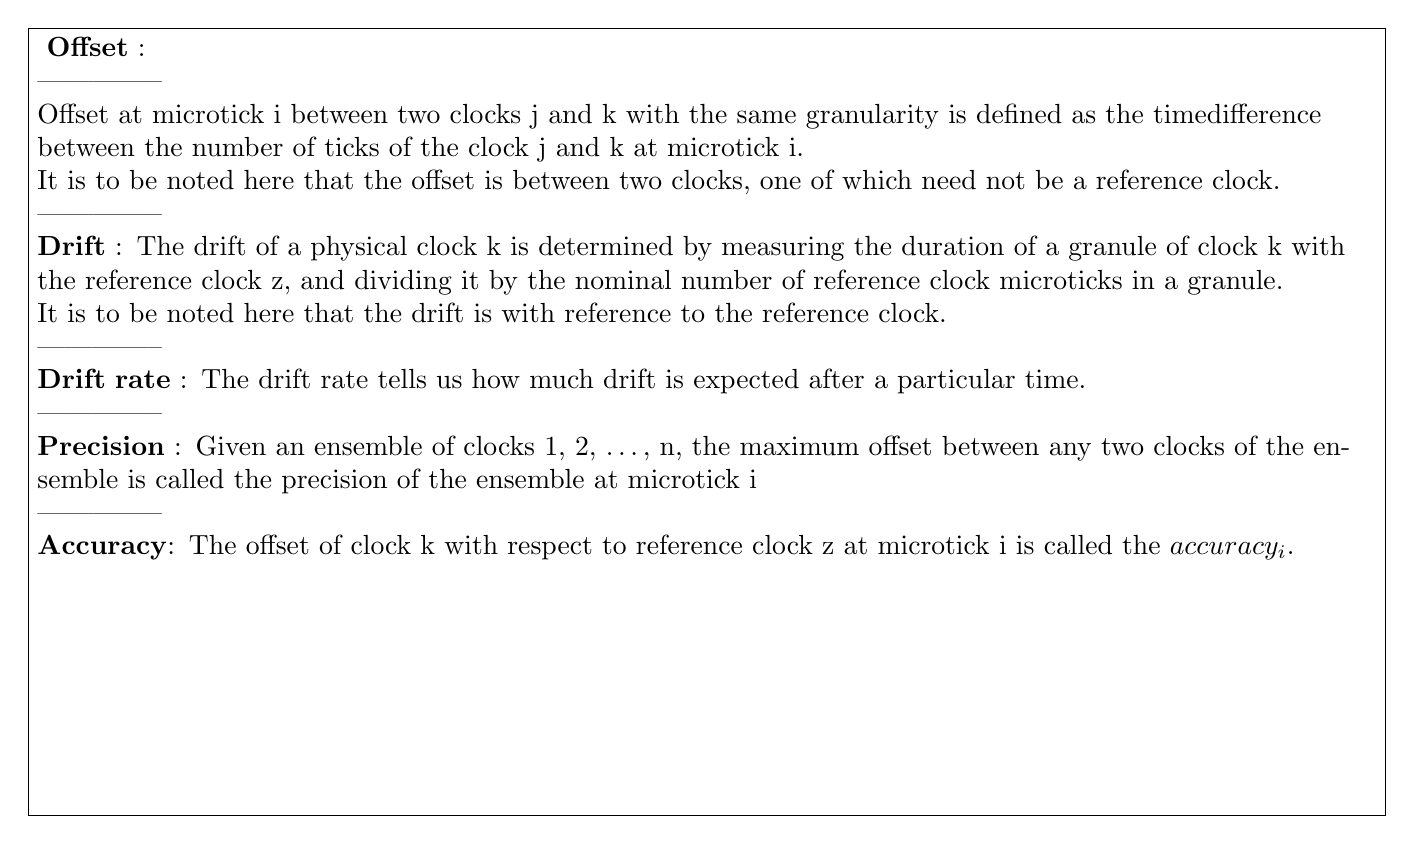
\begin{tikzpicture}
\node (rect) at (0,0) [draw, text width=17 cm, minimum height=10cm]{};
\node[below right, text width=17 cm] at (rect.north west) {
    \lsg{
    \textbf{Offset} : \\
		--------------\\
		Offset at microtick i between two clocks j and k with the same granularity is defined as
		the timedifference between the number of ticks of the clock j and k at microtick i. \\
		It is to be noted here that the offset is between two clocks, one of which need not be a reference clock.\\
		--------------\\
		\textbf{Drift} :  The drift of a physical clock k is determined by measuring the duration of a granule of clock k with the
		reference clock z, and dividing it by the nominal number of reference clock microticks in a granule. \\
		It is to be noted here that the drift is with reference to the reference clock.\\
		--------------\\
		\textbf{Drift rate} : The drift rate tells us how much drift is expected after a particular time. \\
		--------------\\
		\textbf{Precision} : Given an ensemble of clocks {1, 2, …, n}, the maximum offset between any two clocks of the ensemble is called
		the precision of the ensemble at microtick i \\
		--------------\\
		\textbf{Accuracy}: The offset of clock k with respect to reference clock z at microtick i is called the $accuracy_{i}$.
		}
   };
\end{tikzpicture}


\pagebreak

\aufgabe{}{5}


Global time ticks of each node are periodically resynchronized after each resynchronization interval $R_{int}$.

\begin{unteraufgaben}

\item Diagrammatically show the relation between resyncronization interval, precision and drift offset.

\item How much is the clock allowed to drift per second if a latency jitter $\varepsilon$ = 10 ps, 
a resyncronization interval $R_{int}$ = 1 sec and a precision $\pi$ = 10 ns is specified?

\item Considering that 5 clocks are in the system, what is the best precision that can be 
achieved according to the impossibility result?

\end{unteraufgaben}

\begin{tikzpicture}
\node (rect) at (0,0) [draw, text width=17 cm, minimum height=14cm]{};
\node[below right, text width=17 cm] at (rect.north west) {
    \lsg{
    .1\\
		--------------\\
    Diagram\\
    .2\\ 
		--------------\\
    $\pi$ = $\varepsilon$ + 2*$\rho$*$R_{int}$ = 4.995 * 10$^{-9}$ ns/s;\\
    .3\\
		--------------\\
    $\varepsilon$ * ( 1 - $\frac{1}{N}$ ) = 8 ps\\
    }
   };
\end{tikzpicture}


\pagebreak


\aufgabe{}{5}

\begin{unteraufgaben}

\item What is the convergence function $\phi$ in case of the central master algorithm?

\item How does the convergence function $\phi$ change in case there are k malicious clocks 
in a total of N clocks.

\item Calculate the precision $\pi$ based on the fault tolerant sync algorithm for a clock 
constellation with 1 Byzantine clock in a clock ensemble of 5 clocks. 

\end{unteraufgaben}

\begin{tikzpicture}
\node (rect) at (0,0) [draw, text width=17 cm, minimum height=15cm]{};
\node[below right, text width=17 cm] at (rect.north west) {
    \lsg{
    .1 \\
		--------------\\
    $\phi$ = $\varepsilon$ \\
    .2\\
		--------------\\
    $\phi$ = $\frac{k\pi}{(N - 2k)}$ + $\varepsilon$\\
		.3\\
		--------------\\
    $\pi$ = $\frac{(N - 2k )}{( N - 3k )}$*($\tau$ + $\varepsilon$) \\
    $\pi$ = $\frac{(3)}{(2)}$*($\tau$ + $\varepsilon$) \\
    }
   };
\end{tikzpicture}

\pagebreak

\aufgabe{}{5}

A system designer has been assigned a task to calculate the MTTF of human beings. To achieve this, 
50*10$^{4}$ human beings aged 25 years were monitored over one year. It was found that 625 of them failed ( died ) in that year.


\begin{unteraufgaben}

\item Please calculate the  failure rate $\lambda$.

\item Calculate the MTTF.

\item Please analyse your results and explain if this is realistic? If not, what would have 
been a more realistic method to calculate the MTTF?

\end{unteraufgaben}


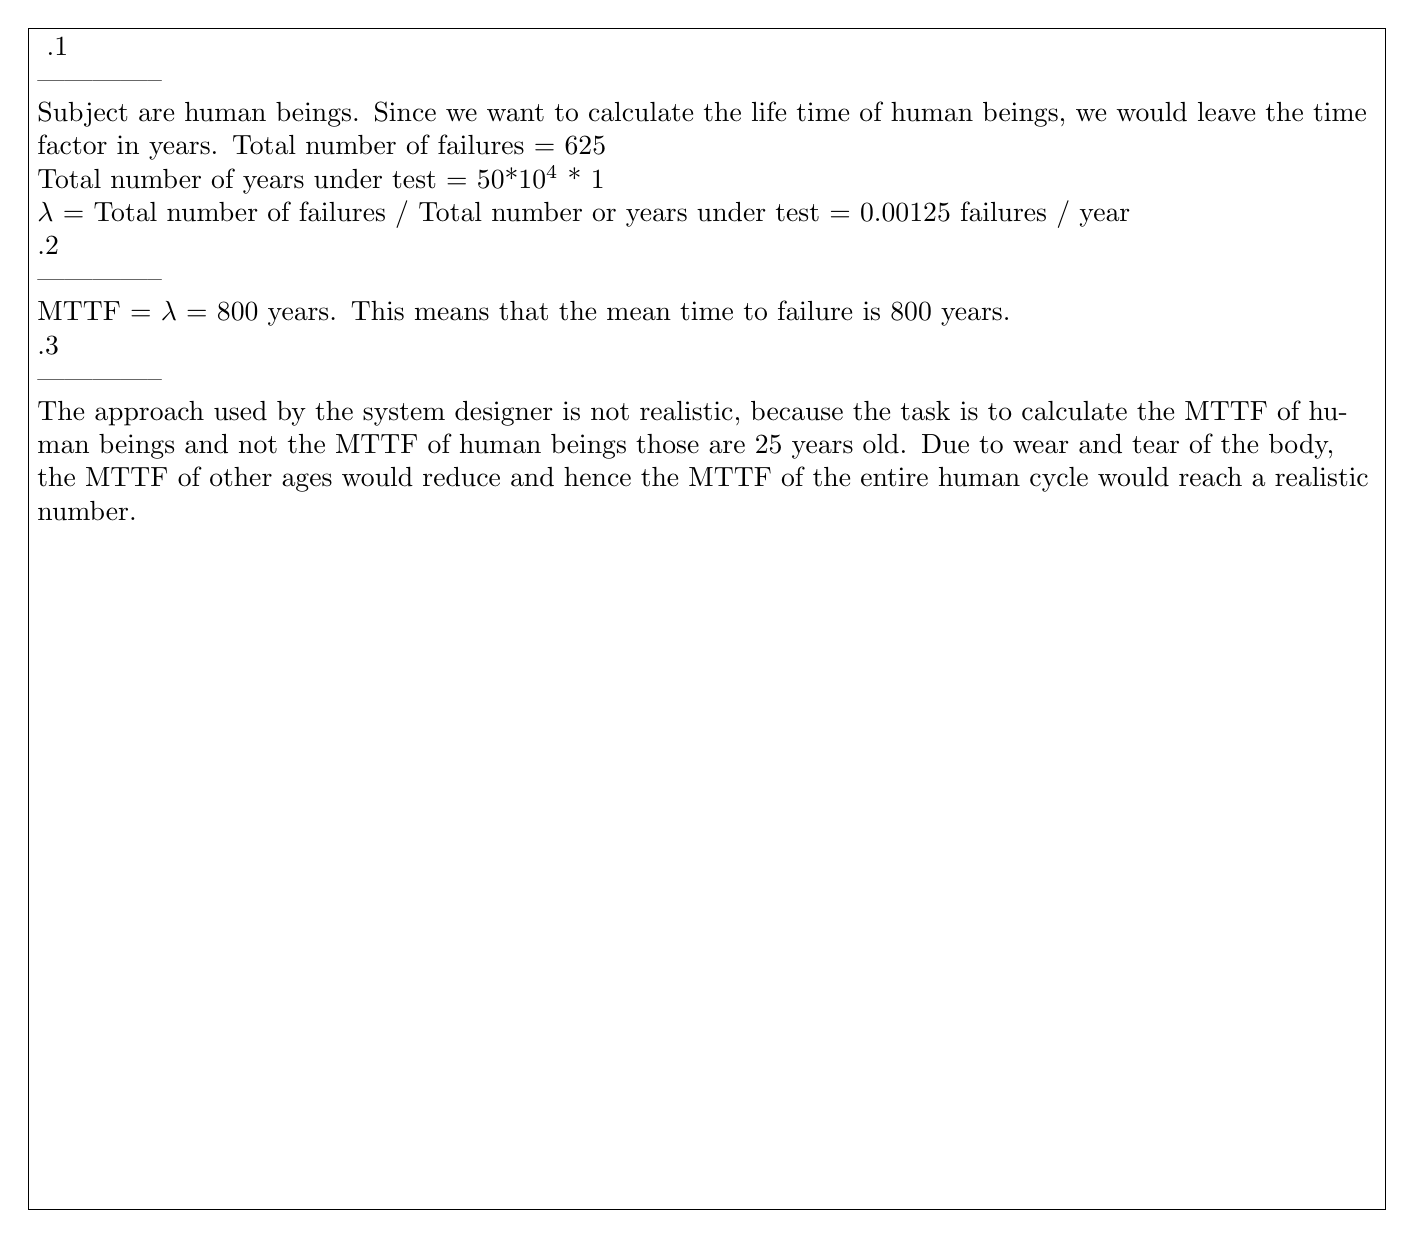
\begin{tikzpicture}
\node (rect) at (0,0) [draw, text width=17 cm, minimum height=15cm]{};
\node[below right, text width=17 cm] at (rect.north west) {
    \lsg{
    .1\\
		--------------\\
    Subject are human beings. Since we want to calculate the life time of human beings, we would leave the
    time factor in years.
    Total number of failures = 625 \\
    Total number of years under test = 50*10$^{4}$ * 1 \\
    $\lambda$ = Total number of failures / Total number or years under test = 0.00125 failures / year \\
    .2\\ 
		--------------\\
    MTTF = $\lambda$ = 800 years. This means that the mean time to failure is 800 years. \\
    .3\\ 
		--------------\\
		The approach used by the system designer is not realistic, because the task is to calculate the MTTF of human beings and not the MTTF of human 
    beings those are 25 years old. Due to wear and tear of the body, the MTTF of other ages would reduce and hence the MTTF of the entire human cycle would
    reach a realistic number.
    }
   };
\end{tikzpicture}

\pagebreak

\aufgabe{}{5}

\begin{unteraufgaben}

\item What are the two main characteristicts of a communication channel? Please explain them.

%\item Given a bandwidth of 10 MBits/sec, a channel length of 200 m and a required protocol efficiency of 90\%, what is the maximum message length in bit that can be implemented by the media access level of a bus system

\item Consider a point-to-point link 2 km in length. At what bandwidth would the propagation delay equal 
transmit time for 100-byte packets? What about 512-byte packets?
Assume the speed of the transmission in the medium =  2*$10^{8}$ m/s,

\end{unteraufgaben}

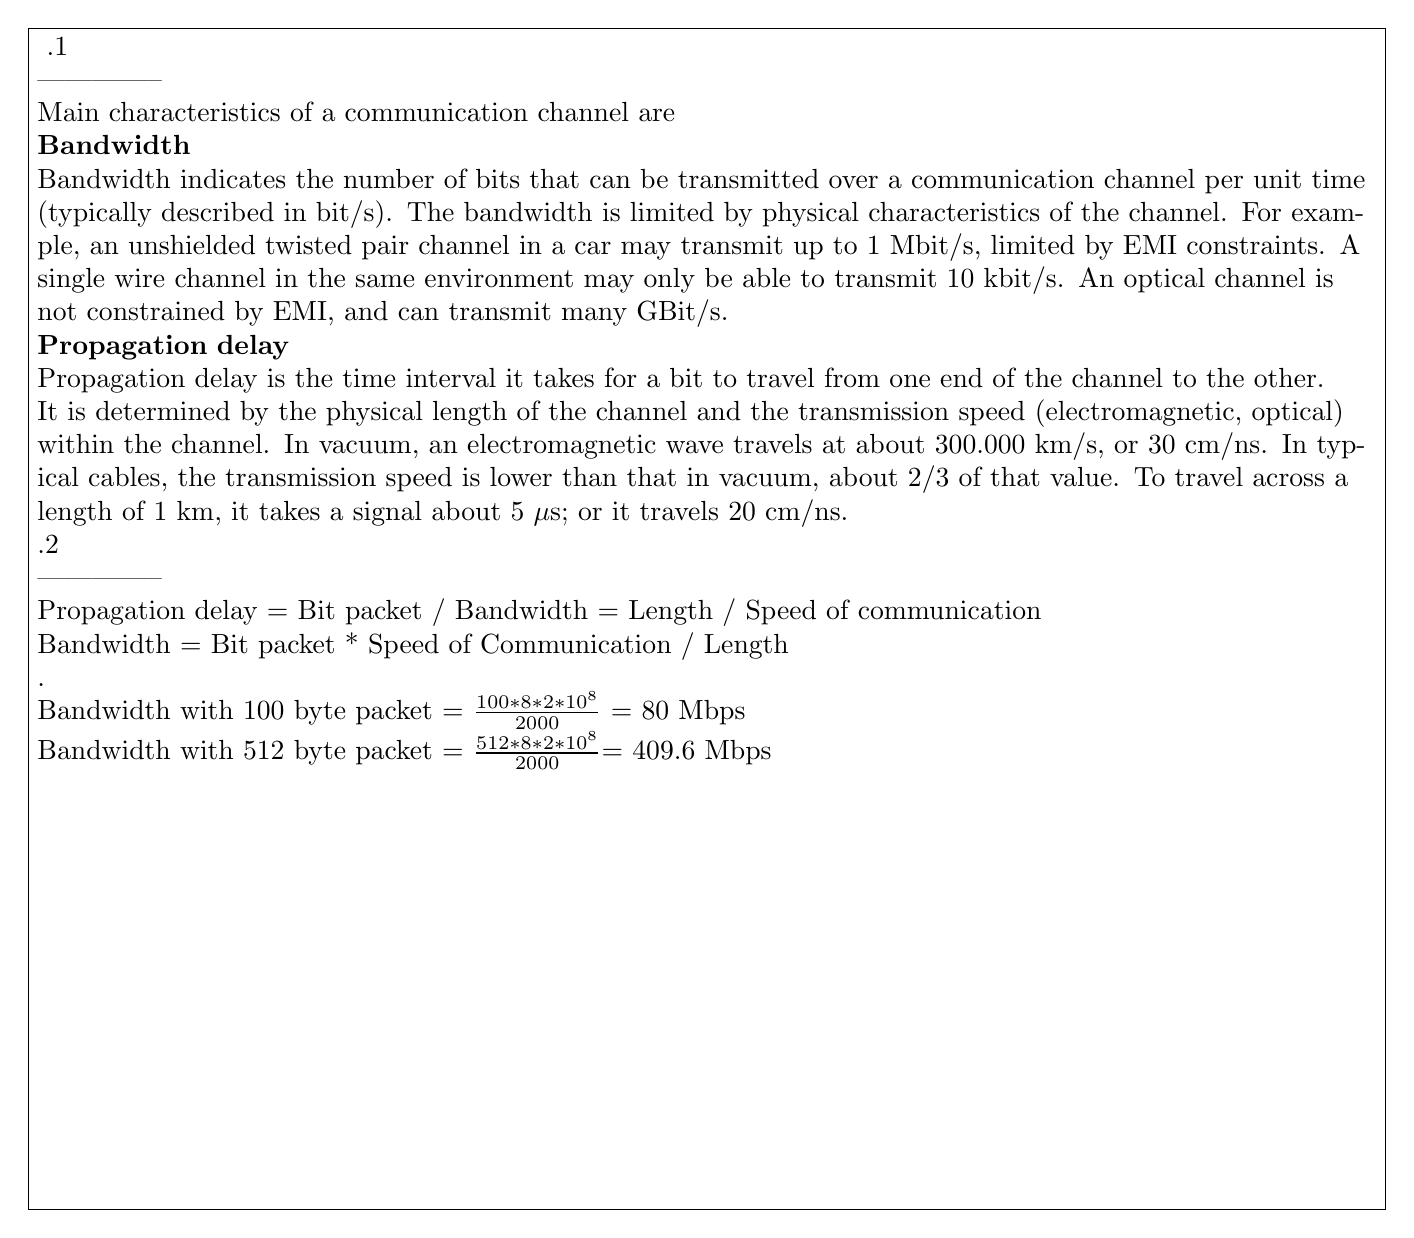
\begin{tikzpicture}
\node (rect) at (0,0) [draw, text width=17 cm, minimum height=15cm]{};
\node[below right, text width=17 cm] at (rect.north west) {
    \lsg{
    .1\\
		--------------\\
Main characteristics of a communication channel are\\
	\textbf{Bandwidth}\\
Bandwidth indicates the number of bits that can be transmitted over a communication channel per unit time (typically described in bit/s). The bandwidth is limited by physical characteristics of the channel. For example, an unshielded twisted pair channel in a car may transmit up to 1 Mbit/s, limited by EMI constraints. A single wire channel in the same environment may only be able to transmit 10 kbit/s. An optical channel is not constrained by EMI, and can transmit many GBit/s.\\
	\textbf{Propagation delay}\\
Propagation delay is the time interval it takes for a bit to travel from one end of the channel to the other.
It is determined by the physical length of the channel and the transmission speed (electromagnetic, optical) within the channel. In vacuum, an electromagnetic wave travels at about 300.000 km/s, or 30 cm/ns. In typical cables, the transmission speed is lower than that in vacuum, about 2/3 of that value. To travel across a length of 1 km, it takes a signal about 5 $\mu$s; or it travels 20 cm/ns.\\
    .2\\
		--------------\\
    Propagation delay = Bit packet / Bandwidth = Length / Speed of communication \\
    Bandwidth = Bit packet * Speed of Communication / Length \\ 
		.\\
    Bandwidth with 100 byte packet = $\frac{100 * 8 * 2 * 10^{8}}{2000}$ = 80 Mbps \\
    Bandwidth with 512 byte packet = $\frac{512 * 8 * 2 * 10^{8}}{2000}$= 409.6 Mbps
    }
   };
\end{tikzpicture}

\pagebreak

\aufgabe{}{10}

One important parameter for many real-time computer programs is the WCET. Please explain why is it 
difficult to determine the WCET of processes in a hard-real time system. State three methods that 
have been advised to determine WCET, and discuss their limitations.

\begin{tikzpicture}
\node (rect) at (0,0) [draw, text width=17 cm, minimum height=15cm]{};
\node[below right, text width=17 cm] at (rect.north west) {
    \lsg{
    Please sketch a model here
    }
   };
\end{tikzpicture}

\pagebreak

\aufgabe{}{5}

Assuming that the start up sequence of the infotainment unit in a car depends on a CAN message sent by the central unit.
Please answer the following questions using timing formulas:

\begin{unteraufgaben}

\item  Given the maximum and minimum communication delay in a system with a local time base, how long after receiving the 
message from the central unit should the infotainment unit wait until the received message can be declared permament?

\item Assuming the above system with a global time base of granularity much smaller than the local time base, how is the  
startup time affected? Please explain your answer.

\end{unteraufgaben}

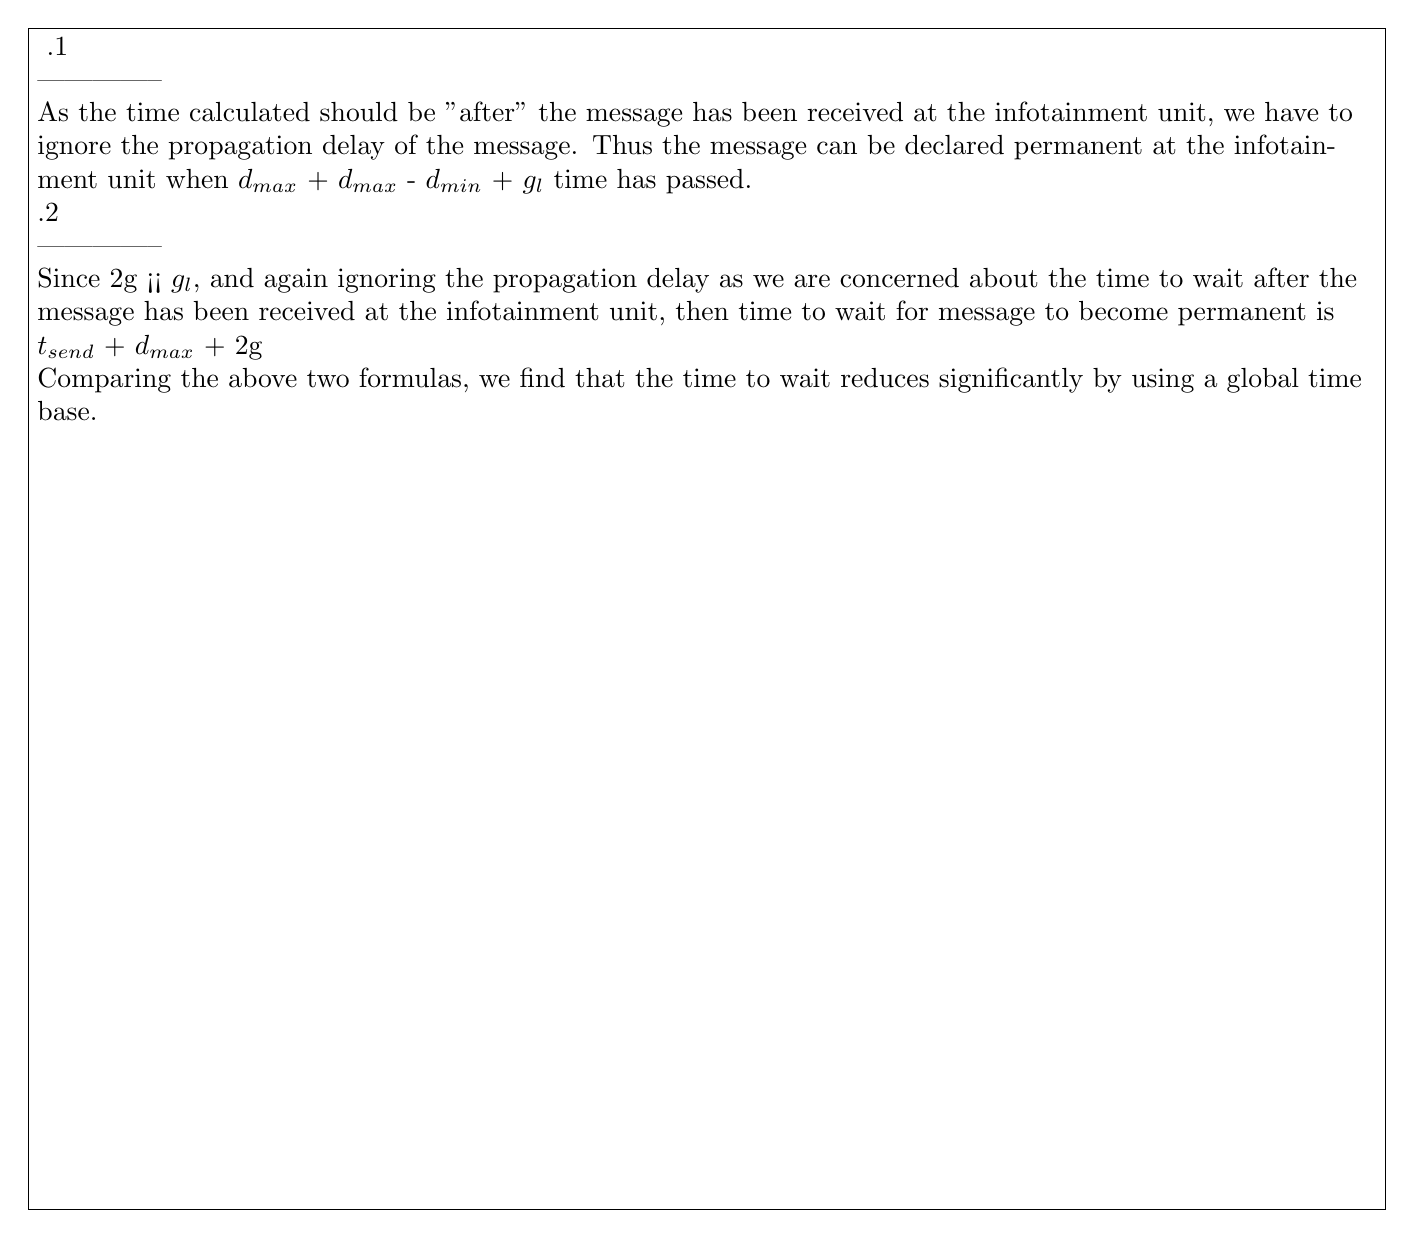
\begin{tikzpicture}
\node (rect) at (0,0) [draw, text width=17 cm, minimum height=15cm]{};
\node[below right, text width=17 cm] at (rect.north west) {
    \lsg{
    .1\\
		--------------\\
    As the time calculated should be "after" the message has been received at the infotainment unit, we have to 
    ignore the propagation delay of the message. Thus the message can be declared permanent at the infotainment unit
    when $d_{max}$ + $d_{max}$ - $d_{min}$ + $g_{l}$ time has passed.\\
    .2\\
		--------------\\
   	Since 2g << $g_{l}$, and again ignoring the propagation delay as we are concerned about the time to wait after the
   	message has been received at the infotainment unit, then time to wait for message to become permanent is \\ 
   	$t_{send}$ + $d_{max}$ + 2g \\
   	Comparing the above two formulas, we find that the time to wait reduces significantly by using a global time base.
    }
   };
\end{tikzpicture}

\pagebreak


\aufgabe{}{5}

Explain the difference between state correction and rate correction for a clock. What are the 
advantages and disadvantages for each method?

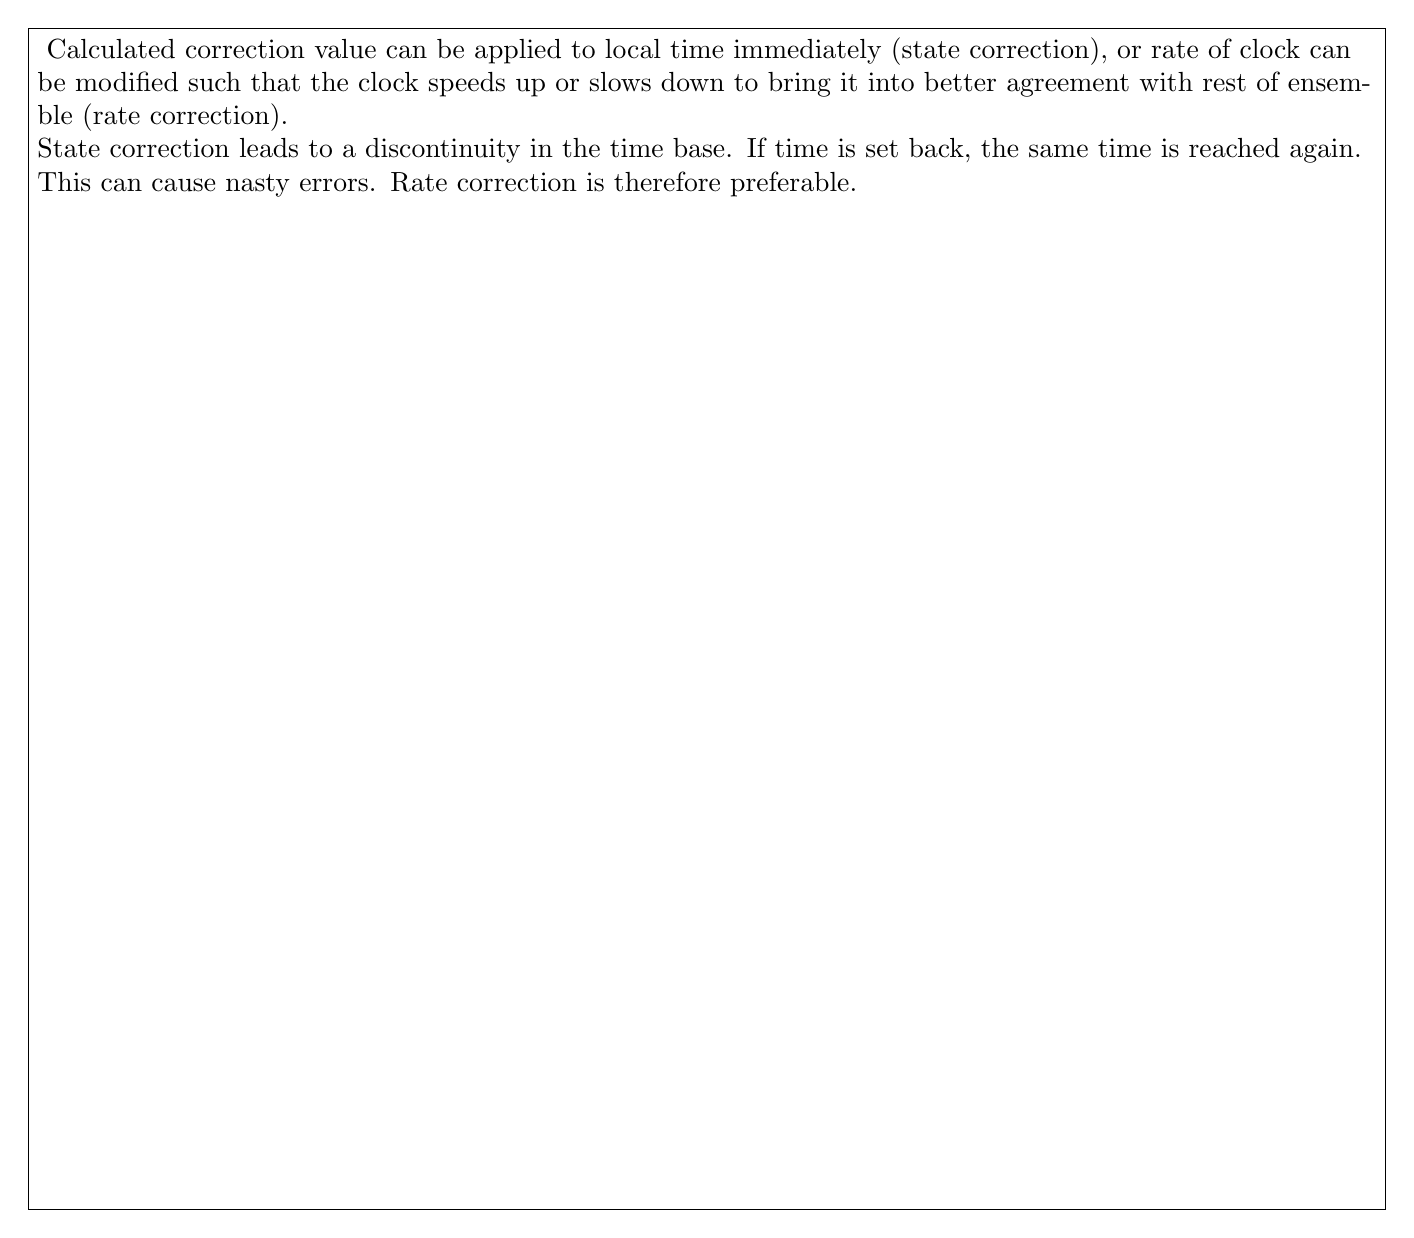
\begin{tikzpicture}
\node (rect) at (0,0) [draw, text width=17 cm, minimum height=15cm]{};
\node[below right, text width=17 cm] at (rect.north west) {
    \lsg{
Calculated correction value can be applied to local time immediately (state correction), or rate of clock can be modified such that the clock speeds up or slows down to bring it into better agreement with rest of ensemble (rate correction).\\
State correction leads to a discontinuity in the time base. If time is set back, the same time is reached again. This can cause nasty errors. Rate correction is therefore preferable.
    }
   };
\end{tikzpicture}

\pagebreak

\aufgabe{}{5}

What is the membership service in the TTP/C protocol? Explain its purpose and briefly explain how it works.

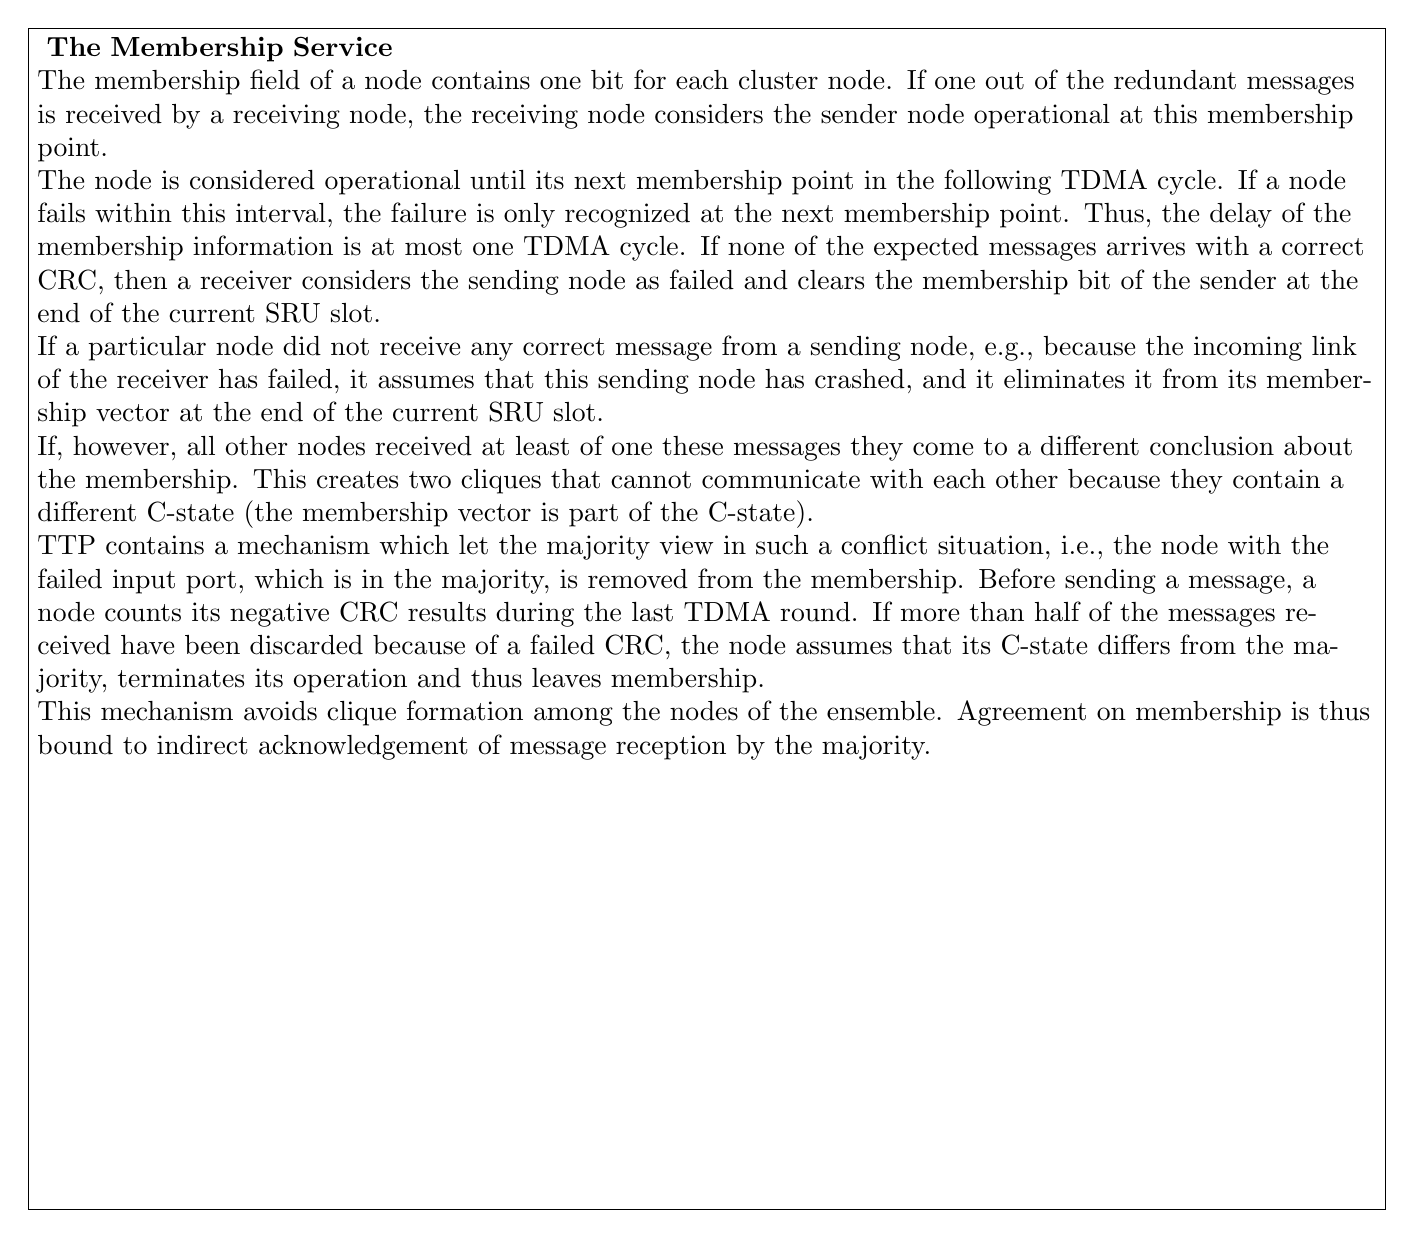
\begin{tikzpicture}
\node (rect) at (0,0) [draw, text width=17 cm, minimum height=15cm]{};
\node[below right, text width=17 cm] at (rect.north west) {
    \lsg{
\textbf{The Membership Service}\\
The membership field of a node contains one bit for each cluster node. If one out of the redundant messages is received by a receiving node, the receiving node considers the sender node operational at this membership point.\\
The node is considered operational until its next membership point in the following TDMA cycle. If a node fails within this interval, the failure is only recognized at the next membership point. Thus, the delay of the membership information is at most one TDMA cycle.
If none of the expected messages arrives with a correct CRC, then a receiver considers the sending node as failed and clears the membership bit of the sender at the end of the current SRU slot.\\
If a particular node did not receive any correct message from a sending node, e.g., because the incoming link of the receiver has failed, it assumes that this sending node has crashed, and it eliminates it from its membership vector at the end of the current SRU slot.\\
If, however, all other nodes received at least of one these messages they come to a different conclusion about the membership. This creates two cliques that cannot communicate with each other because they contain a different C-state (the membership vector is part of the C-state). \\
TTP contains a mechanism which let the majority view in such a conflict situation, i.e., the node with the failed input port, which is in the majority, is removed from the membership. Before sending a message, a node counts its negative CRC results during the last TDMA round. If more than half of the messages received have been discarded because of a failed CRC, the node assumes that its C-state differs from the majority, terminates its operation and thus leaves membership.\\
This mechanism avoids clique formation among the nodes of the ensemble. Agreement on membership is thus bound to indirect acknowledgement of message reception by the majority.\\
    }
   };
\end{tikzpicture}

\pagebreak

\lsg{
Full page solution
}
